\section{Tor § Onion v2}
\begin{frame}{Tor}
    \begin{wrapfigure}{1}{0.2\textwidth}
        \centering
        
\includegraphics[width=0.2\textwidth]{TorLogo}
    \end{wrapfigure}

    La rete Tor è la più famosa implementazione di Onion, le principali migliorie sono state:
    \begin{itemize}
        \item Circuiti telescopici
        \item Utilizzo del protocollo SOCKS
        \item Controllo di congestione
        \item Directory server
        \item Controllo d'integrità end-to-end
    \end{itemize}
    L'obiettivo principale della rete TOR è quello di garantire l'anonimato e scoraggiare eventuali attaccanti, per questo la rete doveva essere semplice da usare, cosi da incrementare il numero di nodi. \\
\end{frame}

\subsection{Network Design}
\begin{frame}{Network Design}
    \begin{wrapfigure}{1}{0.2\textwidth}
        \centering
        \includesvg[width=0.3\textwidth]{overlayNetwork}
    \end{wrapfigure}

    La rete Tor è una rete che esiste al di sopra delle reti esistenti, per questo viene chiamata \textbf{overlay network}. \\
    I pacchetti che viaggiano nella rete Tor sono chiamati \textbf{celle}, hanno una dimensione fissa 512 bytes, e sono di due tipi:
    \begin{itemize}
        \item \textbf{Control}, gestisce il circuito
        \item \textbf{Relay}, trasporta stream dati
    \end{itemize}
\end{frame}

\begin{frame}{Controllo di congestione}
    Non potendo in una rete Onion cambiare un router quando non è più in grado di gestire il carico, è stato necessario implementare un controllo di congestione che blocca i circuiti o gli stream dati quando questi inviano troppi dati usando due finestre:
    \begin{itemize}
        \item Packaging window, tiene traccia del numero di celle che un OR può inviare all'OP
        \item Delivery window, tiene traccia del numero di celle che un OR può inviare fuori dalla rete
    \end{itemize}
    L'unica differenza tra il controllo a livello di circuito o di stream è la dimensione delle finestre.
\end{frame}

\begin{frame}{Tor Relay}
    La rete TOR si basa su un insieme di nodi gestiti da volontari chiamati TOR Relay, possono essere di tre tipi:
    \begin{itemize}
        \item \textbf{Non-exit Relay}, i nodi interni della rete che a loro volta si dividono in:
        \begin{itemize}
            \item \textbf{Guard Relay}, il primo nodo del circuito
            \item \textbf{Middle Relay}, i nodi intermedi del circuito
        \end{itemize}
        \item \textbf{Exit Relay}, i nodi di uscita della rete Tor, instradano il traffico nella rete comune. Essendo gli unici IP visibili all'esterno sono i più esposti a rischi legali.
        \item \textbf{Bridge Relay}, nodi non pubblici che non possono quindi essere bloccati
    \end{itemize}
    Tutte le informazioni sui Relay esistenti sono visitabili al seguente indirizzo: \url{https://metrics.torproject.org/rs.html}

\end{frame}

\begin{frame}{Directory Servers} 
    I Directory Server sono un sottogruppo di onion router che tracciano i cambiamenti nella \textbf{topologia di rete} e agiscono da \textbf{DNS server} per i servizi onion.
    Mantengono infatti i \textbf{descriptor}, pacchetti generati dai servizi onion criptati con la propria chiave privata, che contengono gli introduction points e la chiave pubblica.\\
    
    Il sistema di generazione di indirizzi onion fornisce un \textbf{meccanismo di sicurezza} per evitare che un malintenzionato possa alterare i descriptor e reindirizzare gli utenti ai propri introduction points, infatti se cosi fosse la chiave pubblica nascosta nell'indirizzo onion non sarebbe in grado di decifrare il descriptor.
\end{frame}

\subsection{Dimostrazione Wireshark}
\begin{frame}{Dimostrazione Wireshark}
    Wireshark ci permette di vedere come viene generata la connessione \textbf{TLS}, in cui il client invia alcune informazioni tra cui la versione TLS, la lista dei Cipher Suite supportati e la chiave pubblica.
    Il proxy riceve poi il Server Hello, ovvero la risposta del server con le relative informazioni di criptografia. \\
    Successivamente Tor usa le informazioni ottenute per stabilire una connessione TLS tra client e server, impedendoci di vedere il traffico dati.
\end{frame}

\begin{frame}
    \begin{figure}[htbp]
        \begin{subfigure}[c]{0.5\textwidth}
            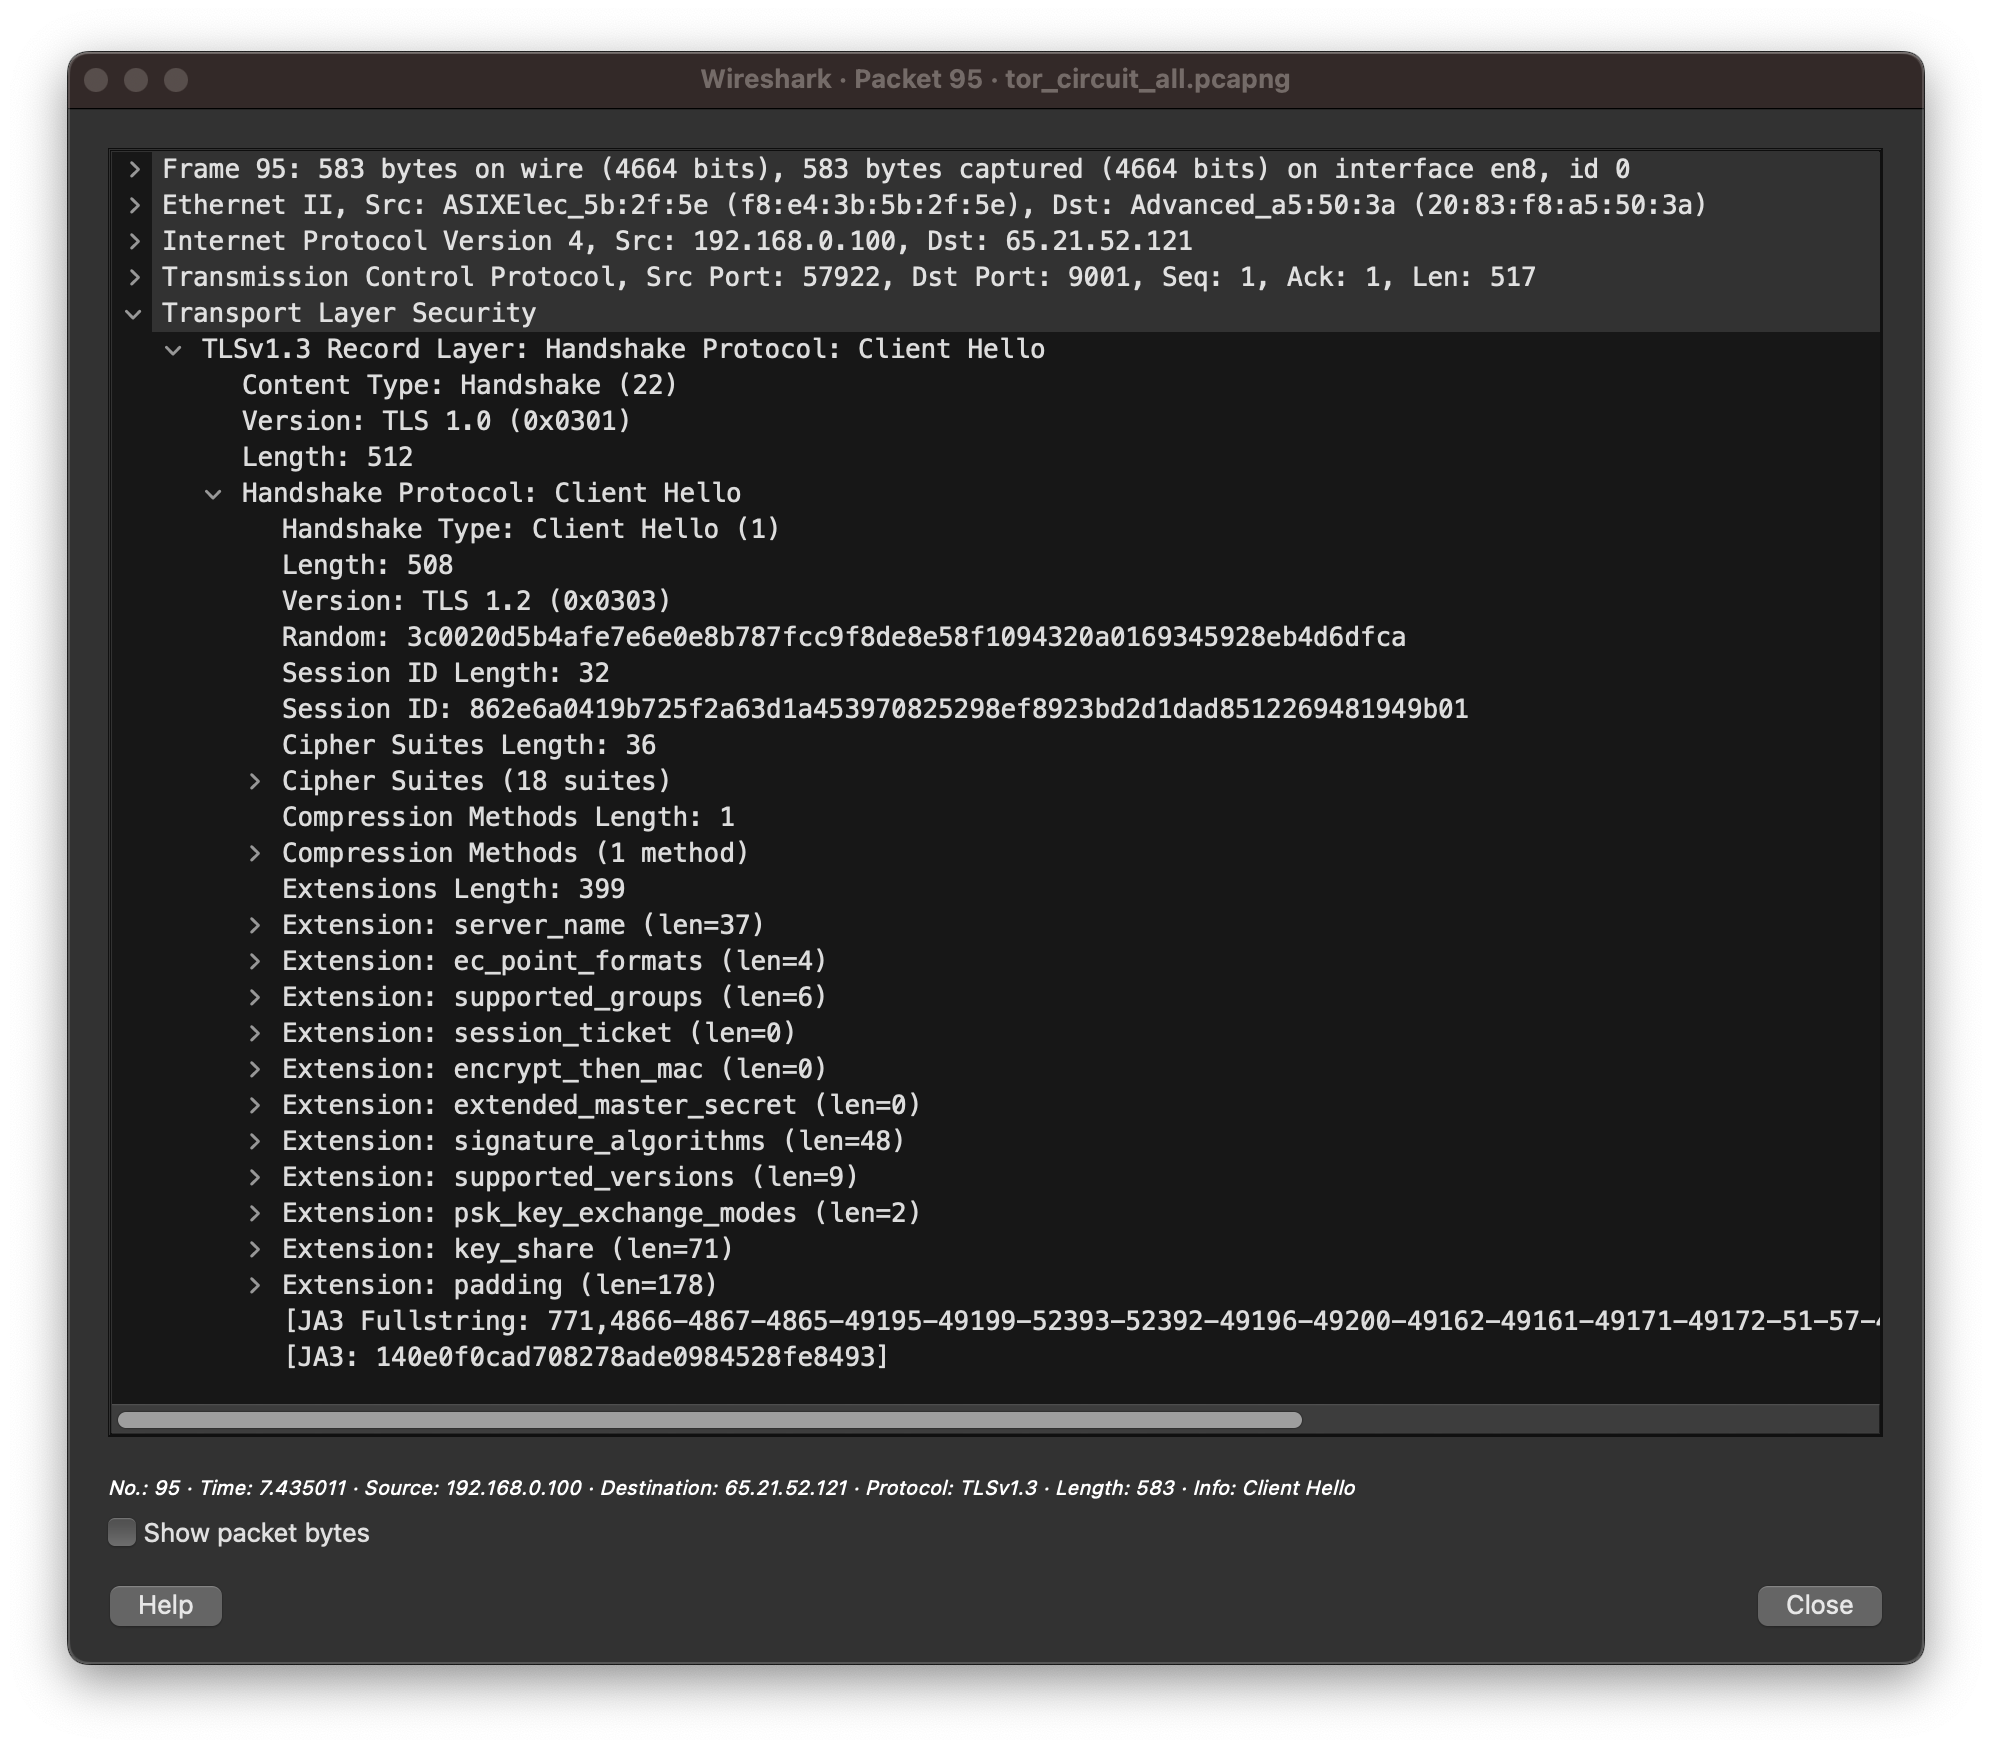
\includegraphics[width=\textwidth]{Wireshark/Client_Hello}
        \end{subfigure}
        \begin{subfigure}[c]{0.49\textwidth}
            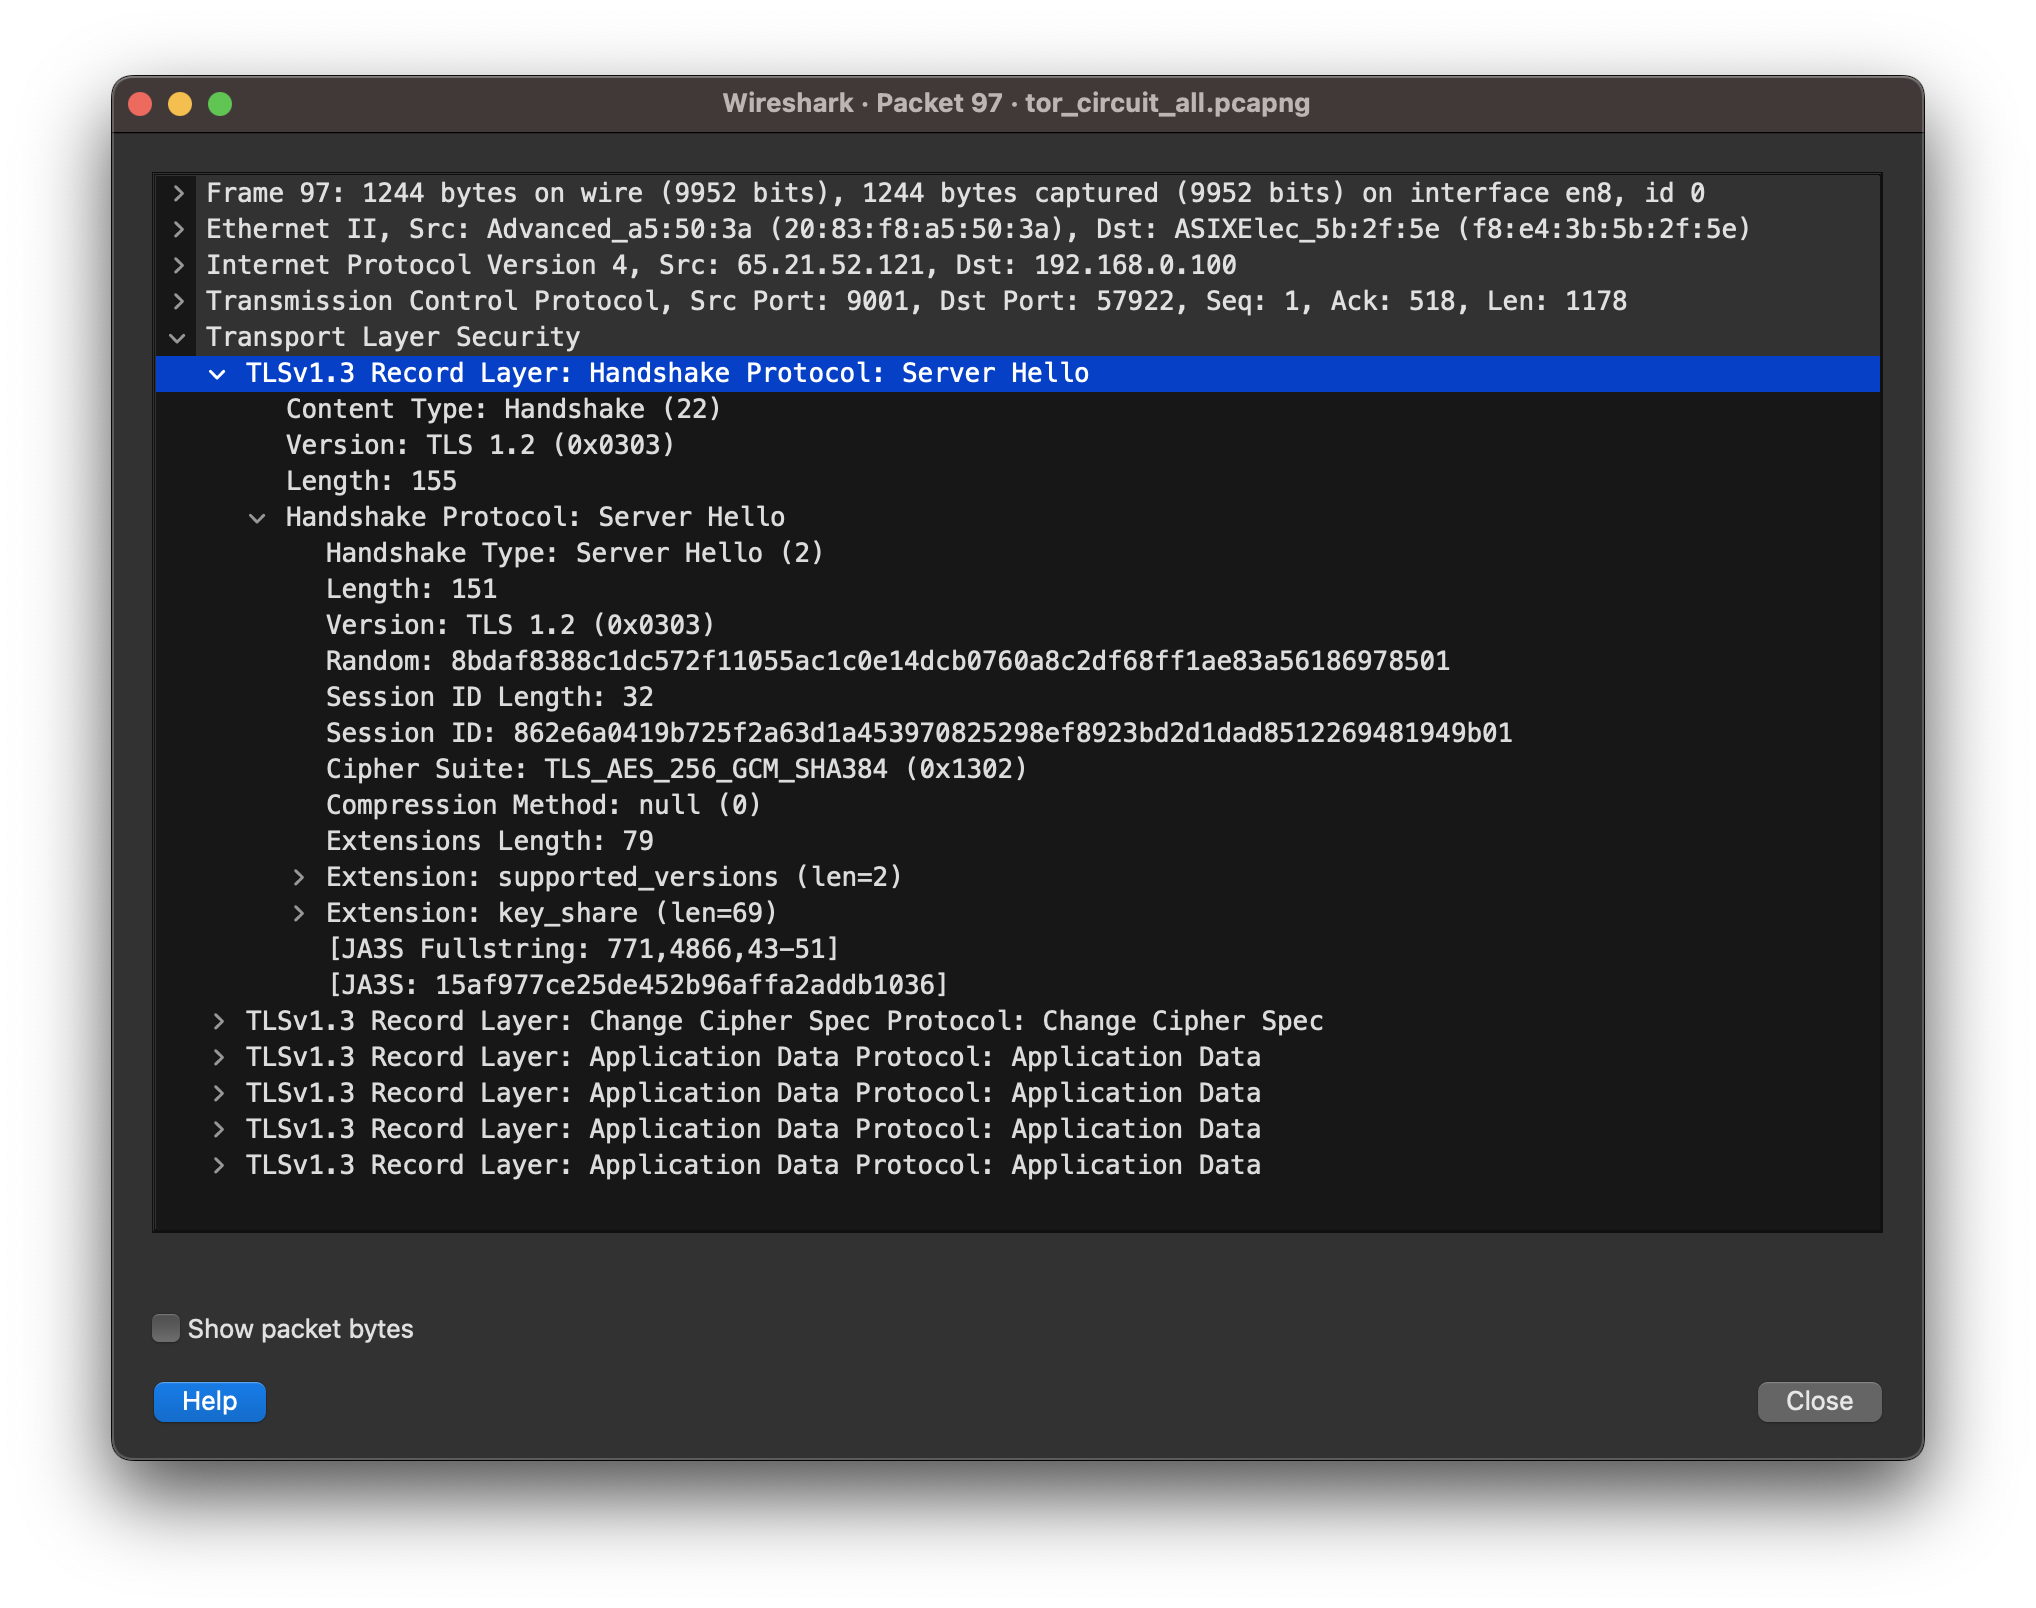
\includegraphics[width=\textwidth]{Wireshark/Server_Hello}
        \end{subfigure}
    \end{figure}
\end{frame}

